\documentclass[9pt, a4paper]{extarticle}

% ----- Packages -----
\usepackage[a4paper, margin=1.5cm, top=1.5cm, bottom=1.5cm]{geometry}
\usepackage[english, bidi=default, provide=*]{babel}

% Use FiraSans to match your other resume and bypass Nix OS font issues natively
\usepackage[sfdefault]{FiraSans}
\renewcommand{\familydefault}{\sfdefault}

\usepackage{graphicx}
\usepackage{xcolor}
\usepackage{paracol}
\usepackage{tikz}
\usepackage{enumitem}
\usepackage{tabularx}
\usepackage{fontawesome5}
\usepackage{calc}
\usepackage[many]{tcolorbox}
\usepackage[hidelinks]{hyperref}
\usepackage{bookmark}
\usepackage{fancyhdr}

% ----- Colors -----
\definecolor{bgdark}{HTML}{2B2B2B}
\definecolor{textwhite}{HTML}{FFFFFF}
\definecolor{textlight}{HTML}{CCCCCC}
\definecolor{stardark}{HTML}{444444}

% ----- Page Style (Fixes black page numbers) -----
\pagestyle{fancy}
\fancyhf{}
\renewcommand{\headrulewidth}{0pt}
\fancyfoot[C]{\color{textlight}\thepage}

% ----- Setup -----
\setlist[itemize]{leftmargin=*, label=\textcolor{textwhite}{\textbullet}, itemsep=3pt, parsep=0pt, topsep=2pt}
\setlength{\parindent}{0pt}
\columnratio{0.37}
\setlength{\columnsep}{2em}

% ----- Custom Commands -----

% Section Headers - Left Column
\newcommand{\cvsectionleft}[1]{
    \vspace{3ex}
    {\large\bfseries\textcolor{textwhite}{\uppercase{#1}}}\par\vspace{0.5ex}
    \textcolor{textwhite}{\rule{3cm}{1pt}}\par\vspace{1.5ex}
    \color{textlight}
}

% Section Headers - Right Column
\newcommand{\cvsectionright}[1]{
    \vspace{1ex}
    {\Large\bfseries\textcolor{textwhite}{\uppercase{#1}}}\par\vspace{2ex}
    \color{textlight}
}

% Timeline Event
\newcommand{\cvevent}[3]{
    \vspace*{1ex}
    % Solid white dot, precisely centered on the 1pt timeline border
    \noindent\makebox[0pt][l]{\hspace*{-14.45pt}\makebox[0pt][c]{\tikz\filldraw[textwhite] (0,0) circle (2.5pt);}}%
    {\large\bfseries\textcolor{textwhite}{\uppercase{#1}}}\par\vspace{0.5ex}
    {\small\textcolor{textlight}{#2}}\par\vspace{1ex}
    {\small\textcolor{textlight}{#3}}\par\vspace{3ex}
}

% Star Ratings
\newcommand{\cvstar}[1]{%
    {\footnotesize
    \foreach \x in {1,...,5}{%
        \ifnum\x>#1\textcolor{stardark}{\faStar}\else\textcolor{textwhite}{\faStar}\fi%
    }%
    }%
}

% Techstack Item 
\newcommand{\staritem}[2]{%
    \par\noindent
    \begin{tabularx}{\linewidth}{@{}p{1.7cm} X@{}}
    \cvstar{#1} & \small\textcolor{textlight}{#2}
    \end{tabularx}\par\vspace{-0.5ex}
}

% Skills Group Item 
\newcommand{\skillgroup}[3]{%
    \par\noindent
    \begin{tabularx}{\linewidth}{@{}p{1.7cm} X@{}}
    \cvstar{#1} & \textbf{\small\textcolor{textwhite}{#2}} \\[-0.5ex]
                & \small\textcolor{textlight}{#3}
    \end{tabularx}\par\vspace{0.5ex}
}

\begin{document}

\pagecolor{bgdark}
\color{textlight}

% ==============================
% HEADER
% ==============================
\noindent
\begin{minipage}[t]{\linewidth - 4cm}
	\vspace{0pt}
	{\Huge\bfseries\textcolor{textwhite}{MAHMOUD AYMAN FAROUK}}\par\vspace{2.5ex}
	{\Large\bfseries\textcolor{textwhite}{Senior DevOps / Platform Engineer}}\par\vspace{0.5ex}
	{\small\textcolor{textlight}{I build reliable systems and enjoy the engineering behind them. I'm a hands-on DevOps/Platform engineer who values automation, reliability, and the craft of building well-designed services that are maintainable and pleasant to operate. I write infrastructure and runtime code---including services and tooling in Go---so I can transform ideas from prototype to production. I love solving problems, tinkering with Linux internals, designing CI/CD and operator-driven automation, and sharing improvements with the community.}}
\end{minipage}%
\hfill
\begin{minipage}[t]{3.5cm}
	\vspace{0pt}
	\centering
	\begin{tikzpicture}
		\clip (0,0) circle (1.75cm);
		\node at (0,0) {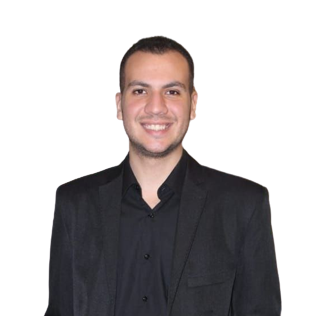
\includegraphics[width=3.5cm]{profile.png}};
	\end{tikzpicture}\par\vspace{1.5ex}
	\begin{tabular}{@{}l@{}}
		\href{https://www.linkedin.com/in/mahmoudk1000}{\textcolor{textwhite}{\faLinkedin \ \ \small LinkedIn}} \\[0.5ex]
		\href{https://github.com/mahmoudk1000}{\textcolor{textwhite}{\faGithub \ \ \small GitHub}}
	\end{tabular}
\end{minipage}

\vspace{3ex}
\noindent\textcolor{textwhite}{\rule{\textwidth}{1pt}}
\vspace{3ex}

% ==============================
% COLUMNS
% ==============================
\begin{paracol}{2}

	% ------------------------------
	% LEFT COLUMN
	% ------------------------------
	\raggedright

	\cvsectionleft{Personal}
	\begin{tabularx}{\linewidth}{@{}p{0.5cm} X@{}}
		\textcolor{textlight}{\faMapMarker} & \small Cairo, Egypt                \\
		\textcolor{textlight}{\faEnvelope}  & \small mahmoud.a.asran@outlook.com \\
		\textcolor{textlight}{\faPhone}     & \small +20 109 179 4795            \\
		\textcolor{textlight}{\faGlobe}     & \small mahmoudk1000.github.io      \\
	\end{tabularx}

	\cvsectionleft{Languages}
	\textbf{\textcolor{textwhite}{Arabic}} {\small [Native]}\par\vspace{1ex}
	\textbf{\textcolor{textwhite}{English}} {\small [Fluent]}\par\vspace{1ex}
	\textbf{\textcolor{textwhite}{German}} {\small [Advanced]}

	\cvsectionleft{Certifications}
	{\small
		\textbf{\textcolor{textwhite}{Associate Cloud Engineer}}\par
		Google Cloud [Feb 2026 -- Feb 2029]\par\vspace{1.5ex}
		\textbf{\textcolor{textwhite}{Certified Solutions Architect}}\par
		AWS [Sep 2026 -- Sep 2029]
	}

	\cvsectionleft{Education}
	{\small
		\textbf{\textcolor{textwhite}{B.Sc. Computer Science}}\par
		Alexandria University [09/2019 -- 06/2023]\par\vspace{0.5ex}
		Grade: Good\par\vspace{1.5ex}
		\textbf{\textcolor{textwhite}{Linux \& DevOps Engineer Training}}\par
		ITI [07/2022 -- 08/2022]\par\vspace{0.5ex}
		Grade: Excellent
	}

	\cvsectionleft{Techstack}
	\staritem{5}{Kubernetes / OpenShift}
	\staritem{5}{Terraform}
	\staritem{5}{Docker}
	\staritem{5}{Linux Internals}
	\staritem{4}{Go (Golang)}
	\staritem{4}{Nix / Nixpkgs}
	\staritem{4}{Ansible}
	\staritem{4}{Prometheus / ELK}
	\staritem{4}{Python / Bash}

	\cvsectionleft{Skills}
	\skillgroup{5}{Cloud}{Azure, GCP, AWS, OpenStack}
	\skillgroup{5}{Containerization}{Kubernetes, OpenShift, Docker}
	\skillgroup{5}{IaC}{Terraform, Ansible, Nix}
	\skillgroup{5}{CI/CD}{GitHub Actions, Azure DevOps, Jenkins}
	\skillgroup{4}{Observability}{Prometheus, ELK, EFK}
	\skillgroup{4}{Programming}{Go, Python, Bash, PowerShell}

	\cvsectionleft{Strengths}
	{\small
		Hands-on Mentality\par\vspace{1ex}
		Linux Internals \& Tinkering\par\vspace{1ex}
		Automation \& SRE Focused\par\vspace{1ex}
		Problem Solving\par\vspace{1ex}
		FOSS Advocate
	}

	% ------------------------------
	% RIGHT COLUMN
	% ------------------------------
	\switchcolumn

	\begin{tcolorbox}[breakable, enhanced, blanker, borderline west={1pt}{0pt}{textwhite}, left=15pt, top=0pt, bottom=0pt, coltext=textlight]

		\cvsectionright{Experience}

		\cvevent{Senior DevOps Engineer}{Atos \textbar{} Cairo, Egypt \textbar{} 09/2026 -- Present}{
			\begin{itemize}
				\item Lead the Kubernetes platform team, managing cluster lifecycle operations, defining architectural direction, and delegating implementation tasks to cross-functional engineers.
				\item Led Atos graduate project sponsorship as technical mentor, guiding interns and training transitioning engineers through onboarding technical courses and workflows.
				\item Designed, implemented, and open-sourced a Kubernetes operator to dynamically set up and scale Azure DevOps pipeline runners, removing CI/CD bottlenecks.
				\item Designed AI-infrastructure and built an LLM-as-a-Service using LiteLLM, vLLM, and NVIDIA NIM, delivering a scalable AI infrastructure serving over 1.3M requests.
			\end{itemize}
		}

		\cvevent{DevOps Engineer}{Atos \textbar{} Cairo, Egypt \textbar{} 07/2024 -- 08/2026}{
			\begin{itemize}
				\item Owned the Azure environment end-to-end, taking full responsibility for all cloud infrastructure.
				\item Selected as the sole engineer requested by the German branch for two separate three-month on-sites in Germany, building team and client trust to deliver critical projects.
				\item Administered and maintained local and cloud-based Kubernetes clusters, ensuring high availability and optimal performance for ongoing workloads.
				\item Built and administered diverse cloud environments with Terraform, setting up OpenShift clusters and managing OpenStack and Proxmox infrastructures, scaling for multiple enterprise customers.
				\item Automated Kubernetes cluster setup and management using PowerShell and Bash, ensuring repeatable setups and reducing manual work.
				\item Operated and improved monitoring tools (Prometheus, Grafana, ELK, EFK) to provide real-time production analytics.
				\item Developed custom Prometheus exporters that enabled white-box monitoring, leading to formal SLIs and SLOs to capture operational indicators and drive core reliability practices.
			\end{itemize}
		}

		\cvsectionright{Projects \& Open Source}

		\cvevent{ACP Cloud Platform}{Infrastructure \& Deployment Automation}{
			Automated diverse cloud environments using Terraform, establishing highly-available OpenShift clusters and managing complex OpenStack infrastructures tailored for enterprise scale and reliability.
		}

		\cvevent{LFP (League de Football)}{Cloud Infrastructure \& CI/CD}{
			Engineered deployment pipelines, infrastructure automation, and robust hosting environments to support the League de Football platform, ensuring high uptime and performance during peak traffic.
		}

		\cvevent{MCIT (Digital Identity)}{Infrastructure Provisioning}{
			Designed and deployed foundational infrastructure and automated CI/CD workflows for the Ministry's Digital Identity initiative, ensuring secure and resilient service operations.
		}

		\cvevent{Nix \& Nixpkgs}{Open Source Contributor \& Maintainer}{
			Long-term reviewer and maintainer in the Nixpkgs ecosystem. Contributed 40+ PRs across various packages and modules, ensuring ecosystem stability, reproducibility fixes, and up-to-date dependencies.
		}

		\cvsectionright{Hobby Projects}

		\cvevent{Felukka (Koptan and Bosla)}{Author \& Maintainer}{
			Developed and maintained open-source tooling centered around the Felukka ecosystem (including Koptan and Bosla). Focused on modernizing workflows and providing extensible tools for the community.
		}

		\cvevent{KARA (Kubernetes Azure-DevOps Runner Autoscaler)}{Author \textbar{} Go, Kubernetes}{
			Authored an open-source Kubernetes operator to manage on-demand Azure DevOps self-hosted runners as CRDs. Features include lifecycle safety via webhooks, secure PAT handling, and PVC-backed workspaces.
		}

	\end{tcolorbox}

\end{paracol}
\end{document}
